%TODO

\section{Introduction}

Wazuh is different than base OSSEC in that it adds functionality (a RESTFul API and rules and decoders) and is easier to install (it uses the ELK stack to gather and preprocess data, while OSSEC leaves that to freedom of the user). Wazuh too is open source and free software.
\begin{figure}[H]
  \centering
	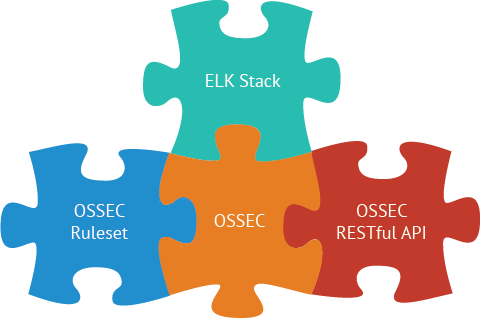
\includegraphics[width=\textwidth]{figuras/wazuh_stack.png}
	\caption{The different technologies that form Wazuh\cite{wazuh_stack}}
\end{figure}
\linej
The most interesting qualities of Wazuh for this project are\cite{wazuh_documentation}: %necessary redundancy
\begin{itemize}
	\item \textbf{Rootkits detection}: Rootkits are commonly used after an attack has suceeded to use the computer of the victim leaving no traces.
	\item \textbf{File integrity monitoring}: It can provide detection of intrusions and can be used to comply with GDPR (General Data Protection Regulation).
	\item \textbf{Scalability and multi-platform}: This means that the work on this project could really be used in real work environments.
	\item \textbf{Configuration management}: The configuration is managed by the Wazuh server (Wazuh manager) and the agents can be grouped, allowing custom, grupal or global gathering and detection for each agent.
	\item \textbf{Multiple sources of data}: The scanned data can be from logs, output of commands or databases. %TODO more?
	\item \textbf{Active response}: An automated remediation to security violations and threats, to mitigate more the posible damage. For example to stop the Internet connection to isolate a compromised system.
	\item \textbf{Improved ruleset}: This reduces the workload of this project, as it can serve as guidance and complement some of the rules and decoders that this project intends to create or modify.
	\item \textbf{Open source, free and easy to contribute to}: This is optional but nice, as it offers a chance to an unexperienced student to contribute in a real and useful project. The project is hosted on Github and Google Groups. In this project the contribution would be to the ruleset\cite{wazuh_ruleset} and not to the core of Wazuh\cite{wazuh} or the documentation\cite{wazuh_documentation2}.
\end{itemize}
\linej
The RESTFul API interacts using OSSEC commands and would be interesting if this project were related to a tool issuing queries to Wazuh, but this is not the case. Anyway it is still something valuable to have as these kind of tools are very common nowadays.


\section{Wazuh architecture}

A Wazuh setup has the next components\cite{wazuh_architecture}:
\begin{itemize}
	\item Wazuh server: Runs the Wazuh manager, API and Filebeat (Filebeat is only necessary in distributed architecture). It collects and analyzes data from deployed agents.
	\item ELK stack: It reads, parses, indexes, and stores alert data generated by the Wazuh server. The ELK stack is flexible, highly configurable and very used in big data.
	\item Wazuh agent: Runs on the monitored host, collecting system log and configuration data and detecting intrusions and anomalies. It talks with the Wazuh server to which it forwards collected data for further analysis.
\end{itemize}
\linej
The main difference with the architecture of OSSEC is the ELK stack, because OSSEC leaves the choice of tools for these functions to the user. ELK stands for the combination of:
\begin{itemize}
	\item Elasticsearch: Gets the data and allows search queries and analysis.
	\item Logstash: Transforms the data to the desired format. This step can make alike data from different log and output formats, trivializing the decoders work.
	\item Kibana: Shows the data in a web browser, with graphs and options like grouping and time interval. This is often easier than to write commands to scan the OSSEC log in the Wazuh server, as the data of interest tends to stay the same.
\end{itemize}
\linej
There are two posible architectures for this setup: having the ELK stack in the same machine that the Wazuh server (singlehost) or in a separated one (distributed). Each has advantages and disadvantages and in this project we will use the singlehost because in our case it does not really matter and is easier to set up and more efficient.
\begin{figure}[H]
  \centering
	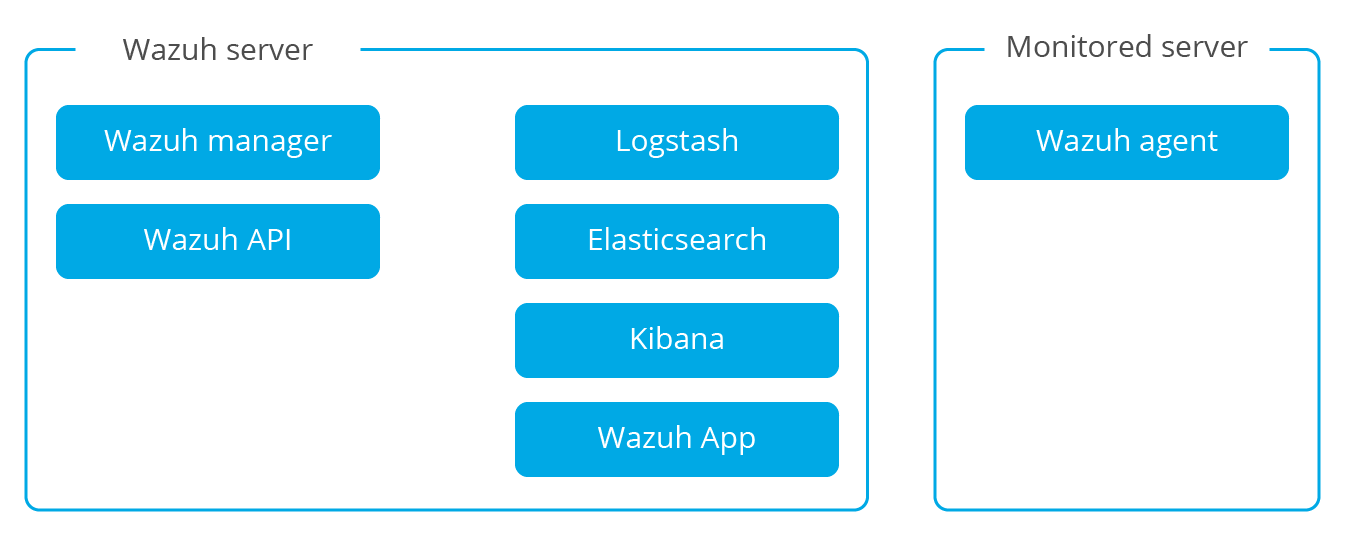
\includegraphics[width=\textwidth]{figuras/wazuh_singlehost.png}
	\caption{Singlehost architecture}
\end{figure}

\begin{figure}[H]
  \centering
	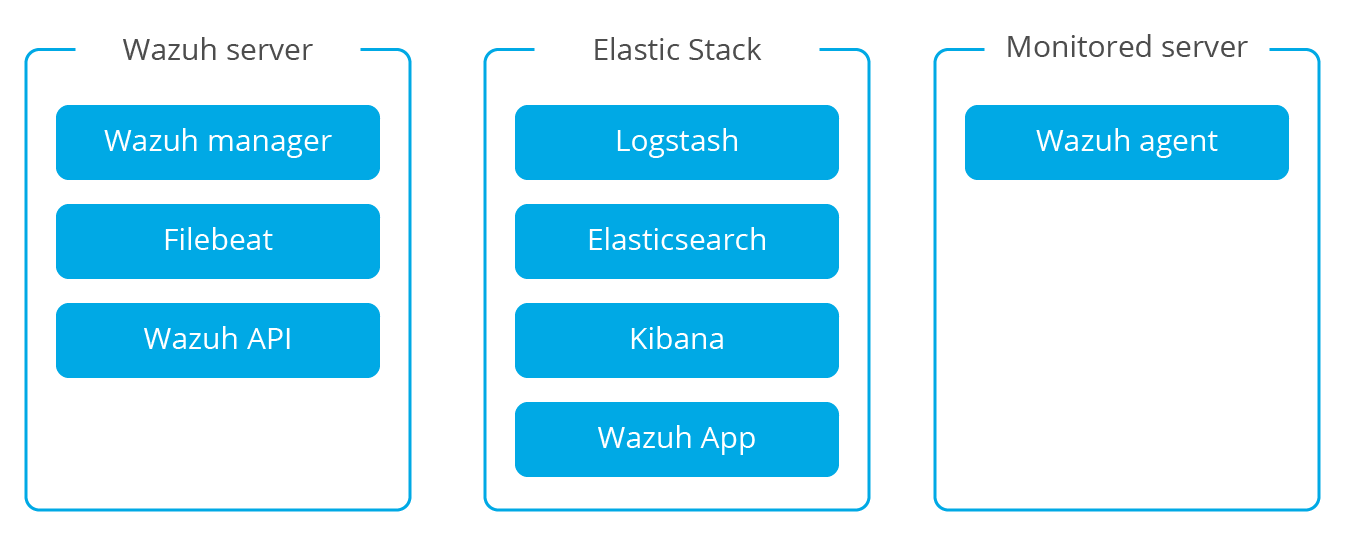
\includegraphics[width=\textwidth]{figuras/wazuh_distributed.png}
	\caption{Distributed architecture}
\end{figure}




\section{Rules and decoders}
